%!TEX encoding = UTF-8 Unicode
% !TeX spellcheck = en_GB
%%%%%%%%%%%%%%%%%%%%%%%%%%%%%%%%%%%%%%
\chapter{Constraints on the Higgs properties }\label{chap:HiggsConstr}
%%%%%%%%%%%%%%%%%%%%%%%%%%%%%%%%%%%%%%
In this chapter, the bounds on the Higgs sector will be discussed. Starting from an overview of the theoretical constraints on the Higgs potential, like the quantum triviality and unitarity. Then, the state-of-the-art experimental results on Higgs properties and couplings measurements will be discussed. However, despite many of the Higgs boson properties have been measured with good accuracy, there are still difficult observables in the Higgs sector and some open problems. These will be addressed at the end of this chapter.   
%%
\section{Theoretical constraints}
 \subsection{Partial-wave unitarity}
Recall that in particle scattering process, the $\mathbf S$ matrix is defined via the relation
\begin{equation}
	\ket{out} = \mathbf{S} \ket{in}
\end{equation}
Since the S-matrix $S$ describes the transition probability, it must satisfy the unitarity condition
\begin{equation}
	\mathbf{S^\dagger S = S S^\dagger }= \mathbb{1},
\end{equation}
in order to have probability / quantum numbers conservation. \\ Moreover, we can remove the identity operator $\irrep{1}$ by defining the operator $T$ such as 
\begin{equation}
	\mathbf{S} =\mathbb{1} + i\mathbf{T} .
\end{equation}
For small coupling, $\mathbf{T}$ is small, enabling the use of perturbation theory. Now, we apply the unitarity condition to find a new relation for $\mathbf{T}$
\begin{align}
	\mathbf{S^\dagger S}  =\mathbb{1} &=(\irrep{1}-i \mathbf{T}^\dagger)(\irrep{1}+i \mathbf{T}) \nonumber \\
	&\Rightarrow -i \mathbf{T}^\dagger + i \mathbf{T} +\mathbf{T}^\dagger \mathbf{T} =0 \\
	&\Rightarrow  \mathbf{T}^\dagger \mathbf{T} = \underbrace{-i(\mathbf{T-T}^\dagger). }_{= 2 \mathfrak{I} (\mathbf{T}) }\nonumber 
\end{align}
With the matrix element given by 
\begin{equation}
	\bra{a}\mathbf{T}\ket{b} = \mathcal M_{ab} (2 \pi)^4 \delta^4(p_a-p_b),
\end{equation}
and using the completeness relations, we define the unity operator in terms of some states $\ket{f}$
\begin{equation}
	\mathbb{1} =  \sum_{f} \prod_{i} \int \frac{d^3p^\prime}{(8 \pi^3)\,2E_i^f}  (2 \pi)^4 \ket{f}\bra{f}.
\end{equation}
Thus, the matrix element should satisfy 
\begin{equation}
	\sum_{f} \prod_{i} \int \frac{d^3p^\prime}{(2 \pi)^3\,2E_i^f} (2 \pi)^4 \delta^4(p_i-\sum_i p^f_i) \mathcal M_{bf} \mathcal M_{af}^* = -i (\mathcal M_{ba}- \mathcal M_{ab}^* ).
\end{equation}.
Here, $f$ denotes any set of intermediate states between $\ket a$ and $\ket b$. For the elastic scattering case, where $a =b$, we arrive at the {\bf Optical Theorem }\footnote{Note that $\mathcal M_{af}$ is diagonalisable since $T$ is normal as a result from the S-matrix unitarity.}

\begin{equation}
	\sum_{f}  \int d\Phi_n(p_a,p_i^f)| \mathcal M_{af}|^2 = 2 \mathfrak{I}( \mathcal M_{aa}). 
	\label{opt}
\end{equation}

Where $d\Phi_n(p_a,p_i^f)$ is the $n$-particle phase space, for the $2\to2$ case, the equality is substituted by $\leq$. \\ From now one, we shall only consider the $2\to2$ case  ($\ket{p_1,p_2} \to \ket{k_1,k_2}$) in which we could simplify the phase space further, rewriting the LHS of \eqref{opt} as
\begin{align}
	&\int  \frac{d^3k_1}{(2 \pi)^3\,2E_1} \int  \frac{d^3k_2}{(2 \pi)^3\,2E_2} (2 \pi)^4 \delta^4(p_1+p_2-k_1-k_2)\,| \mathcal M (s,t)|^2 ,\nonumber \\
	&= \frac{1}{16 \pi} \int_{-1}^{1} d(\cos \theta) | \mathcal M (s,t)|^2.
\end{align}
Recall that the relation between the Mandelstam variable $t$, and the scattering angle for the elastic scattering is given by

\begin{equation}
	t = \frac{1}{2} (s-4 m^2)(\cos \theta-1)
\end{equation}
We could expand the matrix element $\mathcal M (s,t)$ in terms of \emph{partial waves}, isolating $s$ from scattering angle dependence
\begin{equation}
	\mathcal M (s,t) = 16 \pi \sum_j (2j+1)a_j P_j(\cos \theta).
\end{equation}
Where $a_j $ are called the $j$th partial wave amplitude, and  $P_j(\cos \theta)$ are the Legendre polynomials 
\begin{equation}
	P_j(z) = \frac{1}{j!}\frac{1}{2^j} {d^j\over dz^j} (z^2-1)^j
\end{equation}
Which satisfies the orthonormality condition
\begin{subequations}
	\begin{align}
		\int_{-1}^{1} dz \,P_j(z) P_k(z) &= \frac{1}{2j+1} \delta_{jk} \\
		P_j(1) &= 1 \,\,\, \forall j.
	\end{align}
\end{subequations}
We hence get for the LHS of \eqref{opt} scattering 
\begin{align}
	&\int  \frac{d^3k_1}{(2 \pi)^3\,2E_1} \int  \frac{d^3k_2}{(2 \pi)^3\,2E_2} (2 \pi)^4 \delta^4(p_1+p_2-k_1-k_2)\,| \mathcal M (s,t)|^2 ,\nonumber \\
	&= \frac{1}{16 \pi} \int_{-1}^{1} d(\cos \theta) \left[ 16 \pi \sum_j (2j+1) a_j(s) P_j(\cos \theta)\right] \times \nonumber\\ & \qquad \left[ 16 \pi \sum_k (2k+1) a_k^*(s) P_k(\cos \theta)\right], \nonumber \\
	&\Rightarrow \; = 32 \pi \sum_j (2j+1)| a_j(s)|^2.
\end{align}
And the RHS of \eqref{opt}
\begin{equation}
	2 \mathfrak{I}( \mathcal M_{aa}) = \underbrace{2 \mathfrak{I}( \mathcal M(s,0))}_{\text{$t$ is integrated out.}} = 32 \pi  \sum_j (2j+1) \mathfrak{I} (a_j(s)). 
\end{equation}
Otherwise large cancellations needed, $a_j(s)$'s are hierarchal. Thus, we could compare the partial wave amplitudes term-by-term 

\begin{equation}
	| a_j(s)|^2 \leq \mathfrak{I} (a_j(s)) \;\;\; \Rightarrow \mathfrak{R} (a_j(s))^2+ \mathfrak{I} (a_j(s))^2 \leq \mathfrak{I} (a_j(s))
\end{equation}
%\begin{figure}[h!]
%	\centering
%	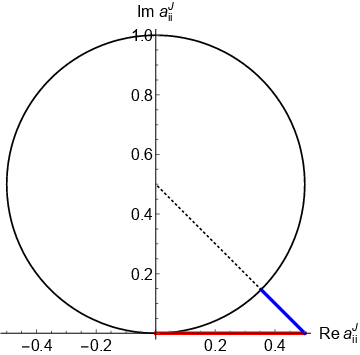
\includegraphics[width = 0.4\textwidth]{Argand}
%	\caption{An Argand diagram illustrating the unitarity circle that the partial wave amplitude need to lie on, the figure is from Di Luzio {\it et al.} Eur. Phys. J. C 77 (2017) 30 }
%	\label{unit}
%\end{figure}
Rearrainging terms, we get
\begin{equation}
	\mathfrak{R} (a_j(s)) +\left( \mathfrak{I} (a_j(s))- \frac{1}{2} \right)^2 \leq \frac{1}{4}
\end{equation}
The partial wave amplitude has to lie within the unitarity circle, see figure~\ref{unit} . We use though perturbation theory if the the partial wave amplitude respects the inequality
\begin{equation}
	\mathfrak{R} (a_j(s)) \leq \frac{1}{2}
\end{equation}

\section{Experimental}
We also provide in this appendix the experimental measurements of the signal strengths at the LHC Run II and the CMS projections for the HL-LHC (scenario S2, see \cite{Cepeda:2019klc}) that we used in the fits in this paper. These inputs are summarised in table~\ref{table:resHiggsExp}.
\begin{figure}[t!]
	\begin{center}
		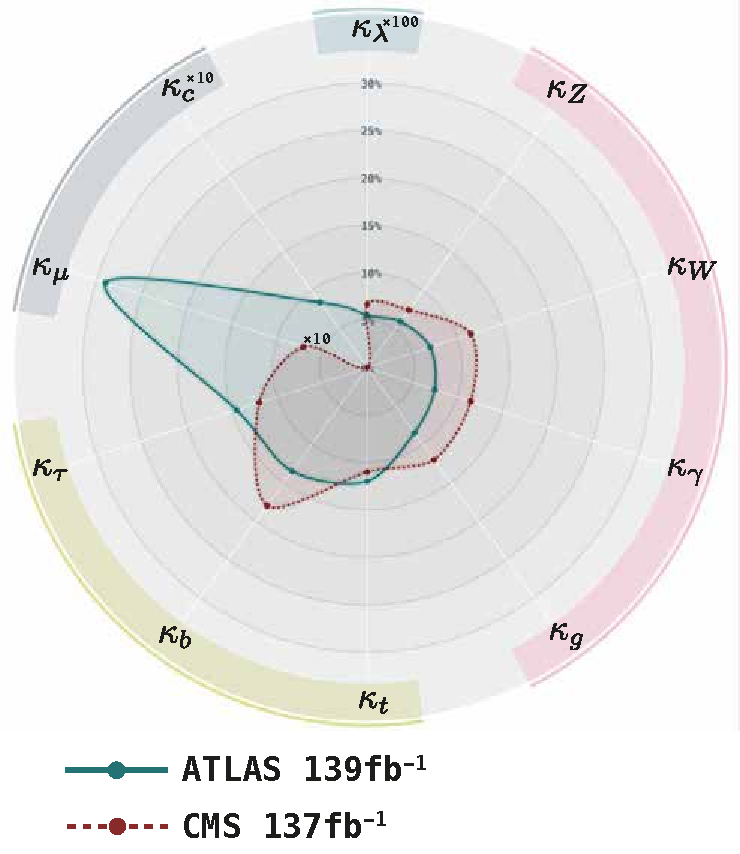
\includegraphics[width=8cm]{figures/kaappa_higgs}
		\caption{ff.\label{fig:higgs_kappa} }
	\end{center}
\end{figure}
\newpage
\begingroup
\thispagestyle{plain}
\begin{table}[htb!]
\centering
\vspace{-1 cm}
 \footnotesize{ 
	{\renewcommand{\arraystretch}{0.75 }%
\begin{tabular}{clccc}
\toprule
\toprule
\multirow{5}{*}{ {\normalsize Production}}  &\multirow{5}{*}{ {\normalsize Decay}}&\multicolumn{2}{c}{ $\mu_{\mathrm{Exp}} \pm \delta \mu_{\mathrm{Exp}}$  (symmetrised)} &\multirow{5}{*}{ {\normalsize Ref.}} \\
%\cmidrule(r){3-4}
&   & { \bf     \scriptsize           LHC Run-II}&{ \bf  \scriptsize HL-LHC}&   \\
\cmidrule(r){3-4}
&   & { \scriptsize                   CMS $137 \, \mathrm{fb}^{-1} $}&  \multirow{2}{*}{CMS $3 \, \mathrm{ab}^{-1}$}&   \\
&   &  { \CG \scriptsize                   ATLAS $139 \, \mathrm{fb}^{-1} $} & &  \\
\midrule
\midrule
\multirow{ 13}{*}{ \normalsize ggF}         & \multirow{2}{*}{$h\to \gamma  \gamma$} & { \scriptsize                  $0.99 \pm 0.12$}& \multirow{2}{*}{$1.000\pm 0.042$}& \multirow{2}{*}{\cite{ATLAS:2020qdt,CMS:2021kom,CMS-PAS-FTR-18-011}}\\
                                           &                                                          &{ \scriptsize                   \CG $1.030 \pm 0.110$}&& \\ 
                                           \cmidrule(r){2-5}
                                           %%%%%%
                                    &  \mr{$h\to Z Z^*$}          & { \scriptsize                  $0.985 \pm 0.115$}&\multirow{2}{*}{$1.000 \pm 0.040$}&\multirow{7}{*}{\cite{ATLAS:2020qdt,CMS:2020gsy,CMS-PAS-FTR-18-011}}  \\
                                     &                                                      &{ \scriptsize                   \CG $0.945 \pm 0.105$}&& \\
                                     \cmidrule(r){2-4}
                                       %%%%%%
                                    &\mr{ $h\to W W^*$}         & { \scriptsize                  $1.285 \pm 0.195$} &\mr{ $1.000 \pm 0.037$} &\\
                                    & &                                            { \scriptsize                   \CG$1.085 \pm 0.185$} & &\\
                                                                         \cmidrule(r){2-4}
                                     %%%%%%
                                    &\mr{ $h\to \tau^+\tau^- $ }         & { \scriptsize                  $0.385 \pm 0.385$} &\mr{ $1.000 \pm 0.055$} &\\
                                 & &                                            { \scriptsize                   \CG$1.045 \pm 0.575$} & &\\
                                 \cmidrule(r){2-5}
                                 %%%%%%

                                  &\mr{ $h\to  b \bar b$  }      & { \scriptsize                 $2.54 \pm 2.44$} &\mr{ $1.000 \pm 0.247$} &\mr{\cite{CMS:2020gsy,CMS-PAS-FTR-18-011}}\\
                               & &                                            { \scriptsize                   \CG--} & &\\
                                 \cmidrule(r){2-5}
                               %%%%%%  %%%%%%   %%%%%%
                                  &\mr{ $h\to  \mu^+ \mu^-$  }      & { \scriptsize      $0.315 \pm 1.815$} &\mr{ $1.000 \pm 0.138$} &\mr{\cite{CMS:2020gsy,CMS-PAS-FTR-18-011} }\\
& &                                            { \scriptsize                   \CG--} & &\\
%%%%%%  %%%%%%   %%%%%%                               
\midrule
\midrule
%\crowcolor
\multirow{13}{*}{ \normalsize VBF}      
                                     %%%%%%
										&\mr{ $h\to \gamma  \gamma$ }         & { \scriptsize                  $1.175 \pm 0.335$ } &\mr{ $1.000 \pm 0.128$} & \mr{\cite{ATLAS:2020qdt,CMS:2021kom,CMS-PAS-FTR-18-011}}\\
										& &                                           { \scriptsize                   \CG$1.325 \pm 0.245$} & &\\
\cmidrule(r){2-5}
%%%%%%                                   
                                     &\mr{$h\to Z Z^*$ }         & { \scriptsize                  $0.62 \pm 0.41$ } &\mr{ $1.000 \pm 0.134$} & \multirow{7}{*}{\cite{ATLAS:2020qdt,CMS:2020gsy,CMS-PAS-FTR-18-011}}\\
                                    & &                                            { \scriptsize                   \CG$1.295 \pm 0.455$} & &\\
                                                                                             \cmidrule(r){2-4}
%%%%%%

                                   &\mr{$h\to W W^*$}         & { \scriptsize                  $0.65 \pm 0.63$ } &\mr{ $1.000 \pm 0.073$} & \\
                                    & &                                            { \scriptsize                   \CG$0.61 \pm 0.35$} & &\\
 \cmidrule(r){2-4}
%%%%%%0
                                   &\mr{$h\to \tau^+\tau^- $}         & { \scriptsize                  $1.055 \pm 0.295$ } &\mr{ $1.000 \pm 0.044$} & \\
& &                                            { \scriptsize                   \CG$1.17 \pm 0.55$} & &\\
\cmidrule(r){2-5}
%%%%%%0                                    
                                    &\mr{$h\to  b \bar b$}         & { \scriptsize                   -- } &\mr{--} & \mr{\cite{ATLAS:2020qdt} }\\
                                    & &                                            { \scriptsize                   \CG$3.055 \pm 1.645$} & &\\
                                    
                                  \cmidrule(r){2-5}
 %%%%%%  %%%%%%   %%%%%%
 &\mr{ $h\to  \mu^+ \mu^-$  }      & { \scriptsize               $3.325 \pm 8.075$} &\mr{ $1.000 \pm 0.540$} &\mr{ \cite{CMS-PAS-FTR-18-011}}\\
 & &                                            { \scriptsize                   \CG--} & & \\                                   
\midrule
\midrule
\multirow{10}{*}{ \normalsize  $t\bar t h$} 
%%%%%%0                                    
&\mr{ $h\to \gamma  \gamma$}         & { \scriptsize                $1.43 \pm 0.30$ } &\mr{$1.000 \pm 0.094$} & \mr{ \cite{ATLAS:2020qdt,CMS:2021kom,CMS-PAS-FTR-18-011} }\\
& &                                            { \scriptsize                   \CG$0.915 \pm 0.255$} & &\\

\cmidrule(r){2-5}

                                    
%%%%%%0                                    
&\multirow{3}{*} { $h\to V V^*$   }         & { \scriptsize              $0.64 \pm 0.64$({\color{Mahogany}$ZZ^*$}) } &{ \scriptsize   $1.000 \pm 0.246$ ({\color{Mahogany}$ZZ^*$}) } & \multirow{8}{*}{\cite{ATLAS:2020qdt,CMS:2020gsy,CMS-PAS-FTR-18-011}}  \\
& &                                            { \scriptsize                   $0.945\pm 0.465$ ({\color{Mahogany} $W W^*$})} & { \scriptsize   $1.000 \pm 0.097$ ({\color{Mahogany} $W W^*$})} &\\
& &                                            { \scriptsize                   \CG $1.735 \pm 0.545$} & { \scriptsize   --}&\\
\cmidrule(r){2-4}                                    

&\mr{$h\to \tau^+\tau^- $}         & { \scriptsize                $0.845 \pm 0.705$} &\mr{ $1.000 \pm 0.149$} & \\
& &                                            { \scriptsize                   \CG $1.27 \pm 1.0$} & &\\
\cmidrule(r){2-4}                                    

&\mr{ $h\to  b \bar b$  }         & { \scriptsize                 $1.145 \pm 0.315$} &\mr{ $1.000 \pm 0.116$} & \\
& &                                            { \scriptsize                   \CG $0.795 \pm 0.595$} & &\\                                                        
\midrule
\midrule
\multirow{9}{*}{ \normalsize $Vh$}        

                      
&\mr{ $h\to \gamma  \gamma$  }         & { \scriptsize   $0.725 \pm 0.295$ } &{ \scriptsize   $1.000 \pm 0.233$ ({\color{Mahogany}$Zh$}) } & \multirow{2}{*}{ \cite{ATLAS:2020qdt,CMS:2021kom,CMS-PAS-FTR-18-011}  }  \\
& &                                            { \scriptsize                   \CG $1.335 \pm 0.315$} & { \scriptsize   $1.000 \pm 0.139$ ({\color{Mahogany} $W^\pm h$})} &\\
\cmidrule(r){2-5}           
%%%%%%0              
                                    
&\mr{ $h\to Z Z^*$    }         & { \scriptsize   $1.21 \pm 0.85$ } &{ \scriptsize   $1.000 \pm 0.786$ ({\color{Mahogany}$Zh$}) } & \multirow{2}{*}{ \cite{ATLAS:2020qdt,CMS:2020gsy,CMS-PAS-FTR-18-011}  }  \\
& &                                            { \scriptsize                   \CG $1.635 \pm 1.025$} & { \scriptsize   $1.000 \pm 0.478$ ({\color{Mahogany} $W^\pm h$})} &\\
\cmidrule(r){2-5}           
%%%%%%0                                         
                                  
 &\mr{ $h\to W W^*$    }         & { \scriptsize   $1.850\pm 0.438$ } &{ \scriptsize   $1.000 \pm 0.184$ ({\color{Mahogany}$Zh$}) } & \multirow{2}{*}{  \cite{CMS:2021ixs,CMS-PAS-FTR-18-011} }  \\
 & &                                            { \scriptsize                   \CG --} & { \scriptsize   $1.000 \pm 0.138$ ({\color{Mahogany} $W^\pm h$})} &\\
 \cmidrule(r){2-5}           
 %%%%%%0                                                                                                            
 &\mr{$h\to  b \bar b$      }         & { \scriptsize  -- } &{ \scriptsize   $1.000 \pm 0.065$ ({\color{Mahogany}$Zh$}) } & \multirow{2}{*}{  \cite{ATLAS:2020qdt,CMS-PAS-FTR-18-011} }  \\
& &                                            { \scriptsize                   \CG $1.025 \pm 0.175$} & { \scriptsize   $1.000 \pm 0.094$ ({\color{Mahogany} $W^\pm h$})} &\\

%%%%%%0                                        
                                    
\midrule
\midrule
\multirow{2}{*}{ \normalsize $Zh$ { \scriptsize {\color{Mahogany} CMS     }   }}    & $h\to \tau^+\tau^- $ & $1.645 \pm 1.485$&\multirow{5}{*}{--} &\multirow{5}{*}{ \cite{CMS:2020gsy} }  \\
& $h\to  b \bar b$       &$0.94 \pm 0.32$&&\\                         
 \cmidrule(r){2-3}    
\multirow{2}{*}{ \normalsize $W^\pm h${ \scriptsize {\color{Mahogany} CMS     }   }}           & $h\to \tau^+\tau^- $ &$3.08 \pm 1.58$&&\\
& $h\to  b \bar b$      & $1.28 \pm 0.41$&&\\                  
\midrule
\midrule
\end{tabular}
}
}
\caption{The experimental single Higgs production and decay rates measurements from the  complete  data of LHC Run II and projections for the HL-LHC. The uncertainties were symmetrised here. The table is published in~\cite{Alasfar:2022zyr}.  }
\label{table:resHiggsExp}
\end{table} 
\endgroup